\chapter{Desenvolvimento} \label{desenvolvimento}

O desenvolvimento do protótipo foi dividido em duas partes. A primeira parte chamada de Hardware que é a montagem do equipamento, formado basicamente por uma placa arduino UNO, sensores e fios de interconexão. No trabalho não foi aplicada nenhuma técnica de soldagem nos equipamentos. A Segunda parte chamada de Software e composta por um código em C ,embarcado no arduino UNO, e um script em Python. A função principal do código em C é capturar os dados dos sensores e ficar esperando caracteres enviados pelo script de Python. Cada caractere corresponde a um dos sensores conectados ao protótipo. O código do script fica armazenado numa estação de trabalho, também tem a responsabilidade de enviar via protocolo MQTT informações para a plataforma ThingSpeak. Essa separação do código em duas partes é útil para a placa arduino que possui memória bem limitada não ficar sobrecarregada. Um código muito extenso pode nem ser embarcado.


Nesse capítulo também e descrito a experiência realizada que tem por objetivo validar a eficiência do protótipo. O experimento compara os dados obtidos na plataforma REDEMET com os coletados pelo protótipo. 

\section{Hardware}

O Hardware da estação meteorológica é composto por sensores: BMP280, DHT22, SV10 e DV10, fios para conexão, dois resistores de 10k$\Omega$, um de resistor de 4.7k$\Omega$, uma protoboard de 480 pontos e um arduino UNO. O diagrama do hardware pode ser visto na figura \ref{fig:hardestacao}.

\begin{figure} [!ht]
    \centering
    \caption{Projeto do Hardware Estação Meteorológica}
    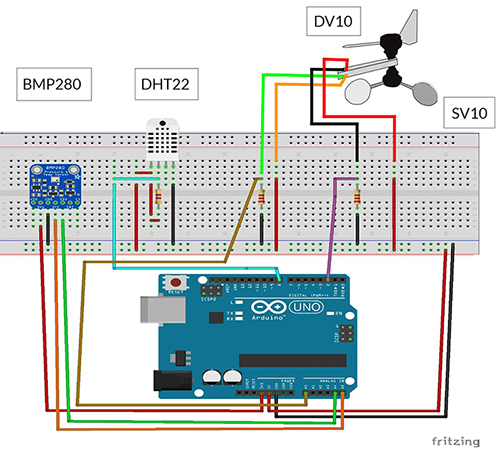
\includegraphics [scale=0.45]{Figuras/estacao_proj_hard.jpg}
    \legend{Elaborado no software Fritzing }
    \label{fig:hardestacao}
\end{figure}

Todos os sensores foram ligados conforme orientação do fabricante. Podemos destacar o sensor BMP280 pela possibilidade de escolher entre: o protocolo de enlace I2C ou SPI. O trabalho optou por utilizar o protocolo I2C por duas razões trabalha em velocidades maiores e a econômia com fios \cite{cinel2017desenvolvimento}. 

Outro detalhe que merece a atenção é o posicionamento da biruta eletrônica e anemômetro. Com o auxílio de uma bússola eles foram colocados de modo que o grau 0º da biruta eletrônica represente o ponto cardeal norte. Esses dois sensores foram colocados em uma altura de 4,56 metros em relação ao chão.

\begin{figure} [!h]
    \centering
    \caption{Hardware Montado}
    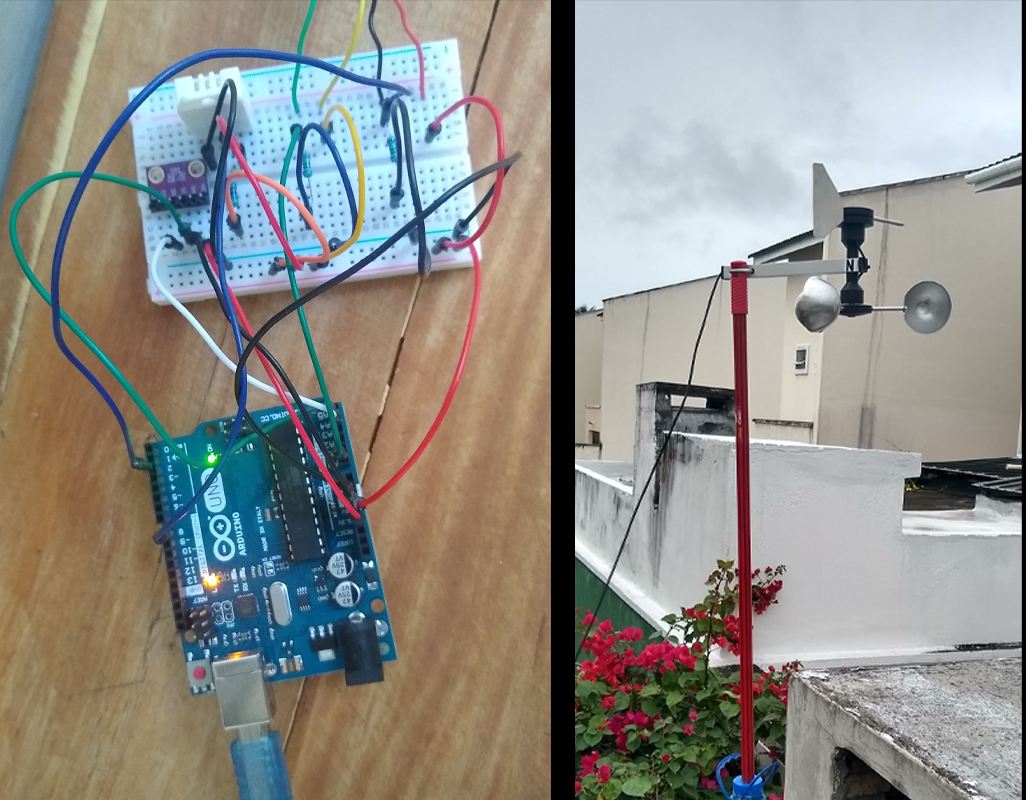
\includegraphics [scale=0.40]{Figuras/Hardware_Estacao.jpg}
    \legend{Fonte: Autoria própria }
    \label{fig:estacao_hardware}
\end{figure}

\section{Software}

Essa parte do desenvolvimento é composta por dois códigos principais um em Python no apêndice \ref{PythonScript} e outro escrito em C no apêndice \ref{CodigoArd}. A divisão além de ajudar no desempenho, melhora a legibilidade do código, isso contribuiu para que a placa arduino utilizasse apenas 32\% da memória interna para armazenamento isso segundo a ferramenta de desenvolvimento arduino IDE.

\subsection{Script em Python}

A primeira ação do código após a importação das bibliotecas necessárias é iniciar as configurações de comunicação serial na mesma porta de operação do arduino com a mesma taxa de transmissão.

No script que está no apêndice \ref{PythonScript} foram deixados explícitos os três modos de conexão da biblioteca do Python para MQTT são eles: usando apenas o protocolo TCP, WebSockets, ou SSL/TLS e WebSockets. A única forma segura de enviar dados é através de SSL/TLS e WebSockets para funcionar é necessário fazer uma configuração na plataforma ThingSpeak e na estação de trabalho que consiste em definir o tipo de certificado e seu caminho na máquina.

Para que a comunicação aconteça com a plataforma é necessário a definição de algumas variáveis como a chave da API de escrita, o endereço MQTT do servidor, e o ID do canal.

Após todas essas configurações as publicações são feitas dentro de um loop infinito onde o tempo de transmissão pode ser configurado. Inicialmente para testes foi estabelecido um valor de 30 segundos. Para exemplificar vou destacar o trecho de código onde o payload é montado e enviado para a plataforma Thingspeak. Dentro do laço perpétuo cada varíavel meterológica tem seu valor coletado através do método realizar\_mensuracao depois o payload é montado conforme a ordem de cadastrado na plataforma Thingspeak e por fim é publicado utilizando o método single do objeto publish do protocolo MQTT. 

\begin{lstlisting}
while(True):

    temperatura = realizar_mensuracao(b't')
    pressao = realizar_mensuracao(b'p')
    umidade = realizar_mensuracao(b'u')
    dir_vento = realizar_mensuracao(b'd')
    vel_vento = realizar_mensuracao(b'a')
    
    tPayload = "field1=" + str(pressao) + "&field2=" + str(umidade) + "&field3=" + str(dir_vento) +  "&field4=" + str(temperatura) +  "&field5=" + str(vel_vento)

    try:
        publish.single(topic, payload=tPayload, hostname=mqttHost, port=tPort, tls=tTLS, transport=tTransport)
        espera(30)

    except (KeyboardInterrupt):
        break

    except:
        print ("Erro ao publicar os dados.") \end{lstlisting}

\subsection{Código embarcado no arduino}

No código do arduino é preciso realizar alguns procedimentos iniciais para a correta inicialização dos sensores. Procedimentos que utilizam bibliotecas de fabricantes para os sensores DHT22 e BMP280. Os sensores DV10 e SV10 apenas necessitam de definições de algumas constantes sem nenhuma chamada de método de biblioteca para configuração.

Para obter as leituras dos sensores DHT22 e BMP280 basta uma chamada de método. O sensor DV10 necessitou de alguns ajustes no método de medição devido à existência de uma variação de 0.15V na saída o que pode gerar imprecisão quando a direção do vento está nas direções de 270 graus e 315 graus. Para realizar o ajuste feito foi realizada 10 leituras do sensor e apenas considerando o valor mediano das medições. O sensor SV10 necessita de 5 segundos para retorna uma leitura isso por que é preciso contar quantas vezes o dispositivo reed switch foi acionado para calcular corretamente o número de rotações por minuto e inferir o daí o valor da velocidade do vento.

Todo o código do arduino pode ser encontrado no apêndice \ref{CodigoArd}. Na figura \ref{fig:acoes_software} pode ser visualizada as principais ações do software no protótipo.

\begin{figure} [!h]
    \centering
    \caption{Principais Ações de Software}
    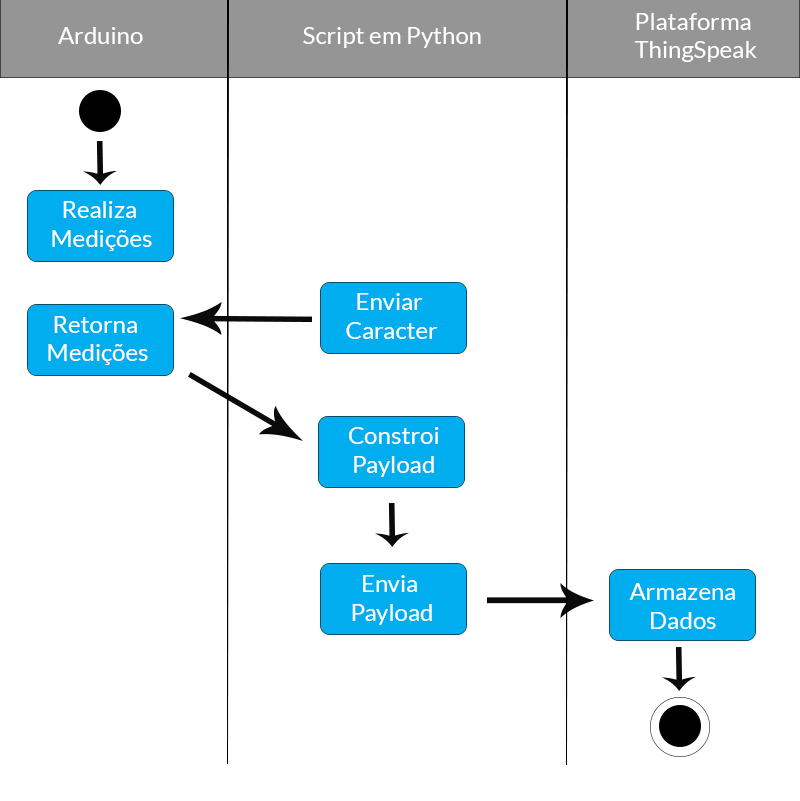
\includegraphics [scale=0.40]{Figuras/fluxo.jpg}
    \legend{Fonte: Autoria própria }
    \label{fig:acoes_software}
\end{figure}

\section{O experimento}

O experimento tem por objetivo produzir resultados para que seja feita uma comparação com a plataforma REDEMET. Ele consiste em deixa o protótipo coletando dados durante três dias e enviando a plataforma ThingSpeak de modo constante e depois será realizado um teste de hipótese para verificar a igualdade das médias das amostras das variáveis.

As variáveis do experimento serão quantitativas contínuas, são elas: temperatura, pressão, umidade relativa do ar, direção do vento e velocidade do vento. Todas os valores coletados serão arrendondados. Na tabela \ref{tab:unidades_medidas} contém informações sobre unidade de medida das variáveis.

\begin{table}[!ht]
\centering
\begin{tabular}{|l|c|}
\hline
\textbf{Variavel}      & \textbf{Unidade de medida} \\ \hline
Temperatura            & Celsius (ºC)               \\ \hline
Pressão                & Hectopascal(hPa)           \\ \hline
Umidade Relativa do Ar & Percentual (\%)            \\ \hline
Direção do Vento       & Graus(º)                   \\ \hline
Velocidade do Vento    & Nó (kt)                    \\ \hline
\end{tabular}
\caption{Fonte: Autoria própria}
\label{tab:unidades_medidas}
\end{table}

O protótipo ira enviar informações das variáveis para a plataforma ThingSpeak a cada 30 segundos. As informações enviadas  podem ser acompanhadas pelo aplicativo disponibilizado pela plataforma. 

\begin{figure} [!h]
    \centering
    \caption{Aplicativo ThingSpeak}
    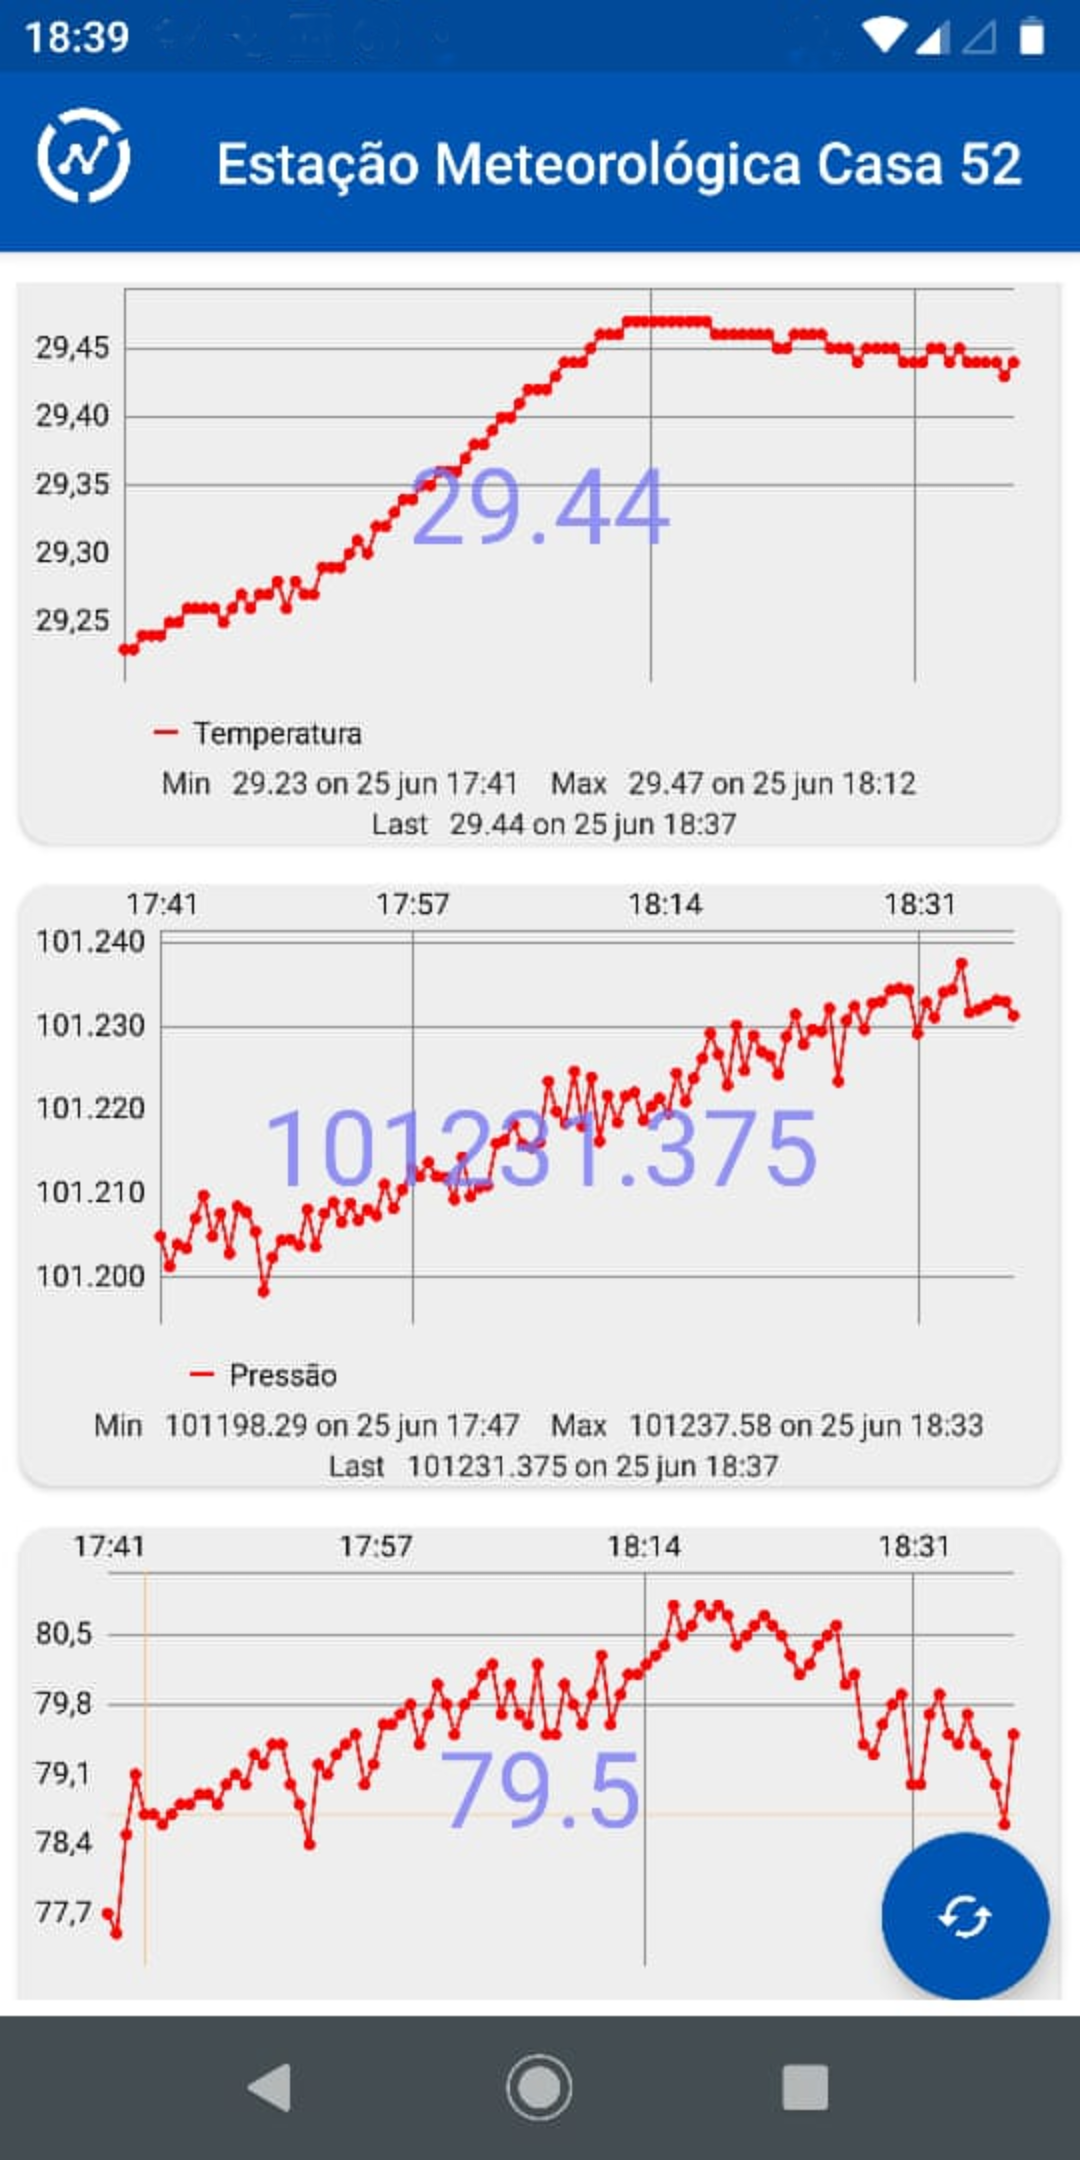
\includegraphics [scale=0.13]{Figuras/img_app.png}
    \legend{Fonte: ThingSpeak App }
    \label{fig:img_app}
\end{figure}

Depois de terminada a etapa de coleta dos dados pelo protótipo é preciso obter dados da plataforma REDEMET. Uma forma de fazer isso e com a API da própria plataforma que permite obter dados meteorológicos a cada hora do dia. No anexo \ref{scriptShell} contém o Shell Script fornecido da plataforma que permite realizar o trabalho de coleta. A plataforma ThingSpeak disponibilizará as informações da amostra do protótipo por meio de um arquivo no formato ".csv".

\subsection{Teste de hipótese}

As amostras coletadas têm tamanhos iguais são 90 observações para cada varíavel. Será utilizado um teste para verificar a igualdade entre as amostras de cada varíavel que consiste em cinco passos são eles:

\begin{enumerate}
   \item Formulação da Hipótese.
   \item Análise da distribuição amostral.
   \item Fixação da significância do teste.
   \item Cálculo da estatística-teste e verificação desse valor com as áreas de aceitação e rejeição do teste.
   \item Aceitação ou rejeição da hipótese.
\end{enumerate}

\subsubsection{Formulação da Hipótese}
As hipóteses serão comuns para todas as variáveis podendo ser definida como:

{\raggedright $\mu_1 \Rightarrow$ A média da variável em análise do protótipo. 
\newline $\mu_2 \Rightarrow$ A média da variável em análise da plataforma REDEMET. 
\newline $ H_0 \Rightarrow$ Hipótese nula.
\newline $ H_1 \Rightarrow$ Hipótese alternativa.

$
\begin{cases}
H_0: \mu_1 = \mu_2 \\
H_1: \mu_1 \neq \mu_1
\end{cases}
$
}

\subsubsection{Análise da distribuição amostral}

\setlength\parindent{2em} A análise da distribuição consiste em verificar se o comportamento das amostras para cada variável. Se segue o padrão da distribuição normal com a utilização de um teste de normalidade pelo módulo scipy.stats.normaltest. Confirmando esse fato será aplicado o teste de cauda superior. Caso uma das distribuições não seja normal será usado o teste estatístico de Wilcoxon. O teste será baseado no trabalho de \cite{d1973tests}. Basicamente o teste irá retornar uma variável chamada de p-valor que será comparado com o nível de significância.

\subsubsection{Fixação da significância do teste}

O nível de significância será o mesmo para todas as variáveis. Ele será utilizado para delimitar a área de aceitação e de rejeição da hipótese.

\begin{figure} [!h]
    \centering
    \caption{Delimitação da Área de rejeição em uma distribuição normal}
    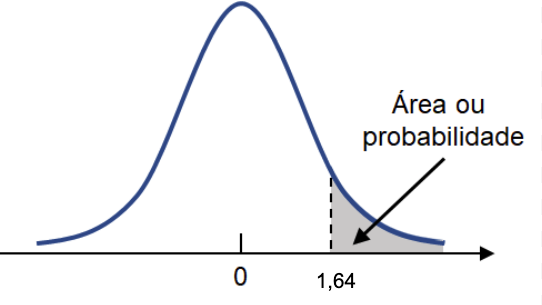
\includegraphics [scale=0.35]{Figuras/nivel_aceitacao.png}
    \legend{Fonte: Autor }
    \label{fig:img_distrNormal}
\end{figure}


\subsubsection{Cálculo da estatística teste e verificação desse valor com as áreas de aceitação e rejeição.}

Nessa etapa do teste aplica a fórmula, através da do módulo DescrStatsW, que tem como objetivo a comparação entre duas amostras para distribuições normais. Conforme fórmula abaixo.

\[\huge Z = \frac{(\bar{x_1} - \bar{x_2})-D_0}{\sqrt{\frac{s_1^2}{n_1} + \frac{s_2^2}{n_2}}}\]

{\raggedright $\bar{x_1} \Rightarrow$ A média da varíavel em análise do protótipo. 
\newline $\bar{x_2} \Rightarrow$ A média da varíavel em análise da plataforma REDEMET. 
\newline $D_0 \Rightarrow$ Diferença entre observações das amostras .
\newline $ s_1^2 \Rightarrow$ Variância da varíavel do protótipo.
\newline $ s_1^2 \Rightarrow$ Variância da varíavel da REDEMET.
\newline $ n_1 \Rightarrow$ número de observações da variável do protótipo.
\newline $ n_2 \Rightarrow$ número de observações da variável da REDEMET.
}

\setlength\parindent{2em}No caso da distribuição não ser classificada como normal será utilizada o módulo Wilcoxon para aplicar a seguinte estatística teste:

{\raggedright$$Z = \frac{T - \mu_T}{\sigma_T}$$

Onde:

$$\sigma_T = \sqrt{\frac{n(n + 1)(2n + 1)}{24}}$$
$$\mu_T = \frac{n(n+1)}{4}$$
$$T = min(R_1, R_2)$$

$ n \Rightarrow$ número de observações da variável do protótipo.
\newline $R_1$ = soma do ranking do grupo 1$n_1$
\newline $R_2$ = soma do ranking do grupo 2$n_2$
}

\subsubsection{Aceitação ou rejeição da hipótese}
\setlength\parindent{2em}
Na última etapa é feita uma comparação do valor encontrado no cálculo da estatística-teste e comparado com o nível de significância. No caso do intervalo de aceitação conter a estatística teste, aceita-se a hipótese nula como estatisticamente válida e rejeita-se a alternativa. Caso contrário é aceito a hipótese alternativa e rejeitado a nula.





